% Intended LaTeX compiler: pdflatex
\documentclass[12pt]{article}
\usepackage[utf8]{inputenc}
\usepackage[T1]{fontenc}
\usepackage{graphicx}
\usepackage{longtable}
\usepackage{wrapfig}
\usepackage{rotating}
\usepackage[normalem]{ulem}
\usepackage{amsmath}
\usepackage{amssymb}
\usepackage{capt-of}
\usepackage{hyperref}
\usepackage[english]{babel}
\usepackage{sbc-template}
\usepackage{url}
\sloppy
\usepackage{listings}
\usepackage{xcolor}
\lstset{
language=C++,
basicstyle=\ttfamily\footnotesize,
keywordstyle=\color{blue}\bfseries,
stringstyle=\color{red},
commentstyle=\color{darkgray}\itshape,
numbers=left,
numberstyle=\tiny\color{gray},
stepnumber=1,
frame=single,
rulecolor=\color{black},
breaklines=true,
captionpos=b
}
\usepackage{graphicx}
\usepackage{tikz}
\usetikzlibrary{positioning, calc, fit, backgrounds, shapes.geometric}
\usepackage{xcolor}
\usepackage{soul}
\usepackage[]{pdfcomment}
\newenvironment{red}{\color{red}}{}
\newenvironment{blue}{\color{blue}}{}
\date{}
\title{A Proposal for a Simulation of PCAD Network Topology Using SimGrid}
\hypersetup{
 pdfauthor={Rayan Raddatz de Matos, Lucas Mello Schnorr},
 pdftitle={A Proposal for a Simulation of PCAD Network Topology Using SimGrid},
 pdfkeywords={},
 pdfsubject={},
 pdfcreator={Emacs 28.2 (Org mode 9.5.5)},
 pdflang={English}}
\begin{document}




\makeatletter
\let\orgtitle\@title
\makeatother

\title{\orgtitle}

\author{
   Rayan Raddatz de Matos\inst{1},
   Lucas Mello Schnorr\inst{1}
   }

\address{
   Institute of Informatics, Federal University of Rio Grande do Sul (UFRGS)\\
   Caixa Postal 15.064 -- 91.501-970 -- Porto Alegre -- RS -- Brazil
   \email{\{rayan.raddatz, schnorr\}@inf.ufrgs.br}}

\maketitle

\begin{abstract}
Simulation is a well-established methodology for evaluating
High-Performance Computing (HPC) systems, ensuring reproducibility and
reduced energy footprints. This work proposes a programmatic network
model of the PCAD infrastructure, a heterogeneous institutional
cluster, using the SimGrid S4U API. Focusing on four core partitions,
we map the physical architecture into a simulated structure and
calibrate the platform properties with experimentation. The main goal
is to enable local researchers to replicate experiments and study
scalability even with limited physical hardware.
\end{abstract}

\section{Introduction}
\label{sec:orga74e203}

Computer systems performance analysis can be done following three
different methods, analytical modeling, simulation or measurement. The
choice of which method to use when performing analysis depends on a
variety of factors such as the time available, the desired accuracy
and several others \cite{jain}. While measurement tends to show the most
accurate results when properly configured, it requires access to the
actual system, which typically leads to higher energy consumption and
limits the ability to extrapolate to new scenarios. On the other hand,
analytical modeling offers great extrapolation capabilities at a
considerably lower energy consumption, but often suffers from low
accuracy results. Simulation acts as a middle term, maintaining good
accuracy with a reduced energy footprint, while also enabling the
exploration of new what-if scenarios. Furthermore, employing
simulations also tackles the problem of the lack of reproducibility in
High-Performance Computing \cite{repro2024}, ensuring a controlled and
reproducible environment for experiments.

Therefore, the simulation of High-Performance Computing (HPC)
infrastructures has become a well-established methodology for
evaluating system behavior. Among the available tools, SimGrid emerges
as a free software capable of simulating several HPC scenarios with
reproducibility and versatility, allowing researchers to simulate
large platforms while maintaining accuracy \cite{simgrid2025}.

In this work, we propose a model of the network of the "Parque
Computacional de Alto Desempenho" infrastructure \cite{LPPD} through the
SimGrid programmatic interface Simgrid For You (S4U). We show
preliminary performance results between the proposed platform created
through simulation and the real cluster.


\noindent
\textbf{Software and Data Availability}. We endeavor to make our analysis
reproducible for a better science. We made available a companion
material hosted in a public GitHub repository at
{\scriptsize\url{https://github.com/rddtz/simgrid-pcad}}.
Our companion contains the source code of this article and the
programmatic description of the platform. We also include instructions
to run the real experiment, simulations and  to recreate the figures.


\section{Related Work}
\label{sec:orgd0a12c5}
\label{org66bbb24}

The evaluation of High-Performance Computing (HPC) systems often
requires balancing accuracy, time, and energy consumption. To achieve
this balance and simultaneously address the lack of reproducibility in
HPC experiments, simulation has become a well-established
methodology. Frameworks like SimGrid offer the versatility needed for
these tasks. Specifically, SimGrid provides the S4U API, which enables
the programmatic creation of complex simulators. Recent works
demonstrate the power of this API for modeling state-of-the-art
environments. As an example, \cite{arthur2025} successfully used the S4U
API to model and simulate the network topology of the Frontier
supercomputer \cite{frontier}. However, while existing works often focus
on modeling massive systems, there is a need to apply and validate
these programmatic creation methodologies in the context of
institutional HPC clusters. Moreover, by creating a validated model of
the PCAD infrastructure, it enable local researchers to easily
replicate experiments and create what-if scenarios, as well as study
scalability even with limited physical hardware.

\section{Platform Proposal and Initial Implementation}
\label{sec:orgc1d7abf}

\subsection{Platform Proposal}
\label{sec:org4dcabad}

Figure  \ref{fig:topology} illustrate the PCAD network
topology. The PCAD infrastructure is composed by four racks and
comports a total of 47 machines separated into 19 different
partitions. Furthermore, the distribution of network capacities varies
across the infrastructure. For instance, while Rack 1, Rack 3, and
Rack 4 utilize 1Gb switches, Rack 2 presents a mixed network capacity,
containing both a 1Gb and a 10Gb switch.  While the complete PCAD
platform is composed of these multiple different partitions, we
initially selected only a few partitions to simulate, these being the
\texttt{cei}, \texttt{draco}, \texttt{tupi}, and \texttt{poti} partitions. The first three partitions have
six nodes each, and the last one has only five. We chose these
partitions as they are the most used ones, aiming to first create a
generic approach that can later be applied to the whole cluster if
necessary.

\begin{figure}[htbp]
\centering
\resizebox{0.8\textwidth}{!}{%
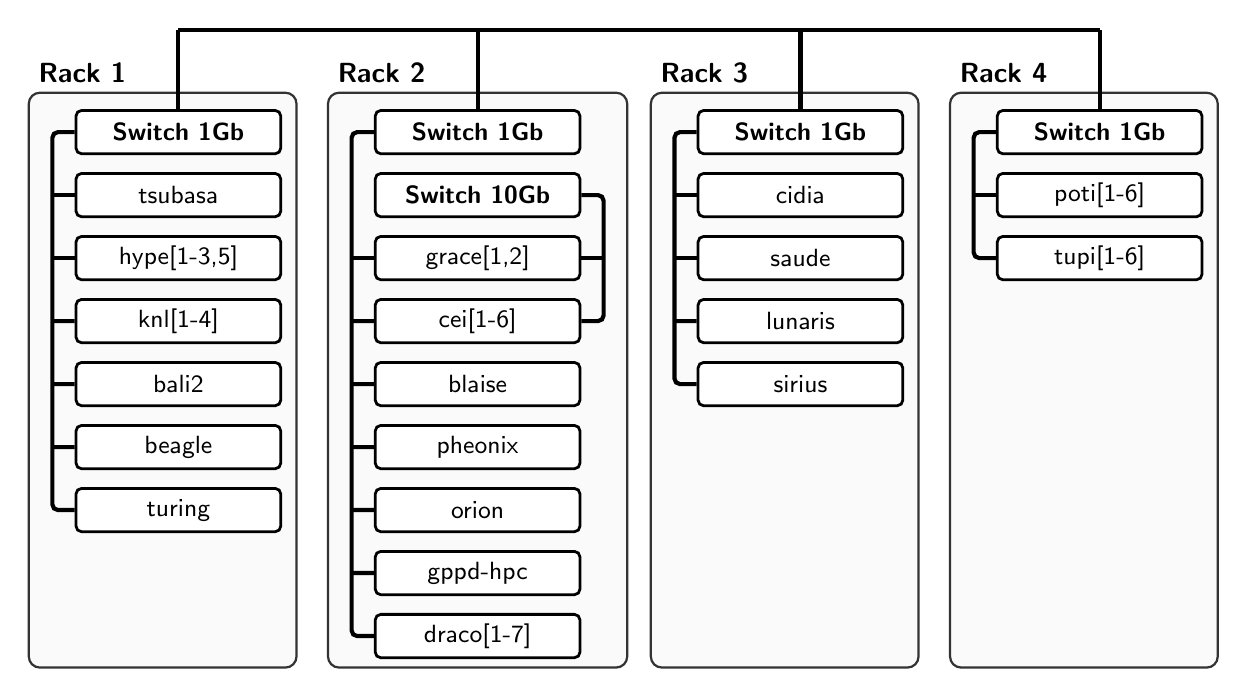
\begin{tikzpicture}[
    % Estilos padronizados e mais fortes
    basenode/.style={rectangle, rounded corners=2pt, draw=black, line width=1pt, minimum width=2.6cm, minimum height=0.55cm, align=center, font=\sffamily\small, fill=white},
    switchnode/.style={basenode, font=\sffamily\small\bfseries},
    rackBg/.style={draw=black!80, line width=0.8pt, fill=black!2, rounded corners=4pt},
    linhaBus/.style={draw, line width=1.5pt, rounded corners=2pt} % Fios bem espessos
]

% ==========================
% COORDENADAS X DOS RACKS (Calculadas para empacotamento perfeito)
% ==========================
\def\XA{0}
\def\XB{3.8}
\def\XC{7.9}
\def\XD{11.7}

% ==========================
% CAIXAS DOS RACKS (Alturas e larguras independentes)
% ==========================
\begin{scope}[on background layer]
    % Rack 1
    \draw[rackBg] (\XA-1.9, 0.5) rectangle (\XA+1.5, -6.8);
    \node[anchor=south west, font=\sffamily\bfseries] at (\XA-1.9, 0.5) {Rack 1};

    % Rack 2
    \draw[rackBg] (\XB-1.9, 0.5) rectangle (\XB+1.9, -6.8);
    \node[anchor=south west, font=\sffamily\bfseries] at (\XB-1.9, 0.5) {Rack 2};

    % Rack 3
    \draw[rackBg] (\XC-1.9, 0.5) rectangle (\XC+1.5, -6.8);
    \node[anchor=south west, font=\sffamily\bfseries] at (\XC-1.9, 0.5) {Rack 3};

    % Rack 4
    \draw[rackBg] (\XD-1.9, 0.5) rectangle (\XD+1.5, -6.8);
    \node[anchor=south west, font=\sffamily\bfseries] at (\XD-1.9, 0.5) {Rack 4};
\end{scope}

% ==========================
% DEFINIÇÃO DOS NÓS
% ==========================
% RACK 1
\node[switchnode] (r1_sw) at (\XA, 0) {Switch 1Gb};
\node[basenode] (r1_n1) at (\XA, -0.8) {tsubasa};
\node[basenode] (r1_n2) at (\XA, -1.6) {hype[1-3,5]};
\node[basenode] (r1_n3) at (\XA, -2.4) {knl[1-4]};
\node[basenode] (r1_n4) at (\XA, -3.2) {bali2};
\node[basenode] (r1_n5) at (\XA, -4.0) {beagle};
\node[basenode] (r1_n6) at (\XA, -4.8) {turing};

% RACK 2
\node[switchnode] (r2_sw1)  at (\XB, 0) {Switch 1Gb};
\node[switchnode] (r2_sw10) at (\XB, -0.8) {Switch 10Gb};
\node[basenode] (r2_n1) at (\XB, -1.6) {grace[1,2]};
\node[basenode] (r2_n2) at (\XB, -2.4) {cei[1-6]};
\node[basenode] (r2_n3) at (\XB, -3.2) {blaise};
\node[basenode] (r2_n4) at (\XB, -4.0) {pheonix};
\node[basenode] (r2_n5) at (\XB, -4.8) {orion};
\node[basenode] (r2_n6) at (\XB, -5.6) {gppd-hpc};
\node[basenode] (r2_n7) at (\XB, -6.4) {draco[1-7]};

% RACK 3
\node[switchnode] (r3_sw) at (\XC, 0) {Switch 1Gb};
\node[basenode] (r3_n1) at (\XC, -0.8) {cidia};
\node[basenode] (r3_n2) at (\XC, -1.6) {saude};
\node[basenode] (r3_n3) at (\XC, -2.4) {lunaris};
\node[basenode] (r3_n4) at (\XC, -3.2) {sirius};

% RACK 4
\node[switchnode] (r4_sw) at (\XD, 0) {Switch 1Gb};
\node[basenode] (r4_n1) at (\XD, -0.8) {poti[1-6]};
\node[basenode] (r4_n2) at (\XD, -1.6) {tupi[1-6]};

% ==========================
% ROTEAMENTO DOS BARRAMENTOS LATERAIS
% ==========================
% Barramento Rack 1
\draw[linhaBus] (r1_sw.west) -- (\XA-1.6, 0) |- (r1_n6.west);
\foreach \i in {1,...,5} { \draw[linhaBus] (\XA-1.6, -0.8*\i) -- (r1_n\i.west); }

% Barramentos Rack 2 (Esquerda: 1Gb / Direita: 10Gb)
\draw[linhaBus] (r2_sw1.west) -- (\XB-1.6, 0) |- (r2_n7.west);
\foreach \i in {1,...,6} { \draw[linhaBus] (\XB-1.6, -0.8*\i - 0.8) -- (r2_n\i.west); }

\draw[linhaBus] (r2_sw10.east) -- (\XB+1.6, -0.8) |- (r2_n2.east);
\draw[linhaBus] (\XB+1.6, -1.6) -- (r2_n1.east);

% Barramento Rack 3
\draw[linhaBus] (r3_sw.west) -- (\XC-1.6, 0) |- (r3_n4.west);
\foreach \i in {1,...,3} { \draw[linhaBus] (\XC-1.6, -0.8*\i) -- (r3_n\i.west); }

% Barramento Rack 4
\draw[linhaBus] (r4_sw.west) -- (\XD-1.6, 0) |- (r4_n2.west);
\draw[linhaBus] (\XD-1.6, -0.8) -- (r4_n1.west);

% ==========================
% LIGAÇÃO SUPERIOR (Backbone alinhado e elevado)
% ==========================
\def\Ybackbone{1.3} % Altura definida para passar bem acima dos títulos
\draw[linhaBus] (r1_sw.north) -- (\XA, \Ybackbone);
\draw[linhaBus] (r2_sw1.north) -- (\XB, \Ybackbone);
\draw[linhaBus] (r3_sw.north) -- (\XC, \Ybackbone);
\draw[linhaBus] (r4_sw.north) -- (\XD, \Ybackbone);
\draw[linhaBus] (\XA, \Ybackbone) -- (\XD, \Ybackbone); % Fio mestre conectando todos

\end{tikzpicture}
}
\caption{Network topology of PCAD.}
\label{fig:topology}
\end{figure}

After defining the platform scope, the SimGrid for You (S4U) C++ API with
SimGrid v4.1 was used to programmatically implement the network
model. The physical architecture was mapped into a hierarchical
simulated structure using S4U's Star Zones. Each rack was therefore
defined as a distinct network zone and within these zones individual
host nodes are instantiated. The modeling explicitly defines hardware
characteristics for each node, including physical core counts and
computational speed measured in Gflops. Network capabilities are
established by attaching dedicated links to each host, specifying
both bandwidth and latency.


\subsection{Platform Calibration Methodology}
\label{sec:orgf293441}

After having a programmatic model of the network topology, the next
stop is to calibrate it. The calibration consist in the execution of
several experiments in the target system to gather information about
its capabilities. The essential information for each hosts are the
host computing power and the host connection bandwidth and
latency. The information about the computing power can be achieved by
various ways, we chose to use the High-Performance Linpack (HPL)
\cite{HPL2003}. For each partition, the HPL was executed 10 times across
two different machines, and the mean result in Gflops was taken as the
speed of a node in that partition. For the network properties, we used
simple network tools such as \texttt{iperf3} for bandwidth and \texttt{ping} for
latency. Official SimGrid material was also used to calibrate the
network and MPI factors for each partition \cite{calibration}.


\section{Preliminary Results}
\label{sec:org4a670e8}
\label{orgce89371}

We used the LULESH proxy app \cite{lulesh}, a common benchmark for MPI
communication and network performance, to evaluate a initial
implementation.  Figure \ref{fig:org7d372c7} show the mean time for
execution of different experiments sizes (represented as a bigger
circle) in function of the number of nodes. Small circles represents
our observations. The time is given by the application as output at
the end of the computation. The black bars centered around the mean
represents the standard error with a CI of 99\%. The figure shows the
results faceted by partition, with the colors identifying where the
execution takes place, in the real cluster (\texttt{real}) or in the SimGrid
(\texttt{sim}). The simulation was executed in a node of the \texttt{cei} partition.


\begin{figure}[!htb]
\centering
\includegraphics[width=1\textwidth]{/tmp/babel-TmQorR/figure9egZHc.pdf}
\caption{\label{fig:org7d372c7}Mean execution time of the LULESH benchmark for different partitions.}
\end{figure}


As observed in the results, there is currently a noticeable gap
between the simulated execution times and the real cluster performance
across the partitions. This initial discrepancy is an expected
behavior during the early stages of modeling a heterogeneous
environment. While the initial calibration successfully captured host
computing power and link limits for some partitions, the complex
behavior of the network requires further refinement. Consequently, the
next necessary step is to perform a deeper, more granular calibration,
particularly focusing on adjusting the network and MPI factors to
accurately simulate communication overhead and contention.

\section{Conclusion}
\label{sec:org24b5d0b}
\label{org2c28c6e}

This work proposed a programmatic methodology to model the
heterogeneous PCAD infrastructure using the SimGrid S4U API. We
established a hierarchical baseline and an initial calibration
workflow. Preliminary results show that while static hardware
capabilities are represented, the network behavior still diverges from
the physical cluster. Future work focus on a iterative fine-grained
calibration of MPI and network parameters.

\section*{Acknowledgements}
We would like to thank the PCAD at INF/UFRGS for making infrastructure
and hardware used in the experiments available. We also acknowledge
the Brazilian National Council for Scientific Technological
Development (CNPq) for their financial support through the PIBIC-UFRGS
scholarship.

\bibliographystyle{sbc.bst}
\bibliography{refs}
\end{document}